\section{Morfologisk analyse af kontrolsystem} \label{Morf - kontrolsystem}

Kontrolsystemet til det mekaniske koncept der ses i figur \ref{fig:Endelig mekaniske koncept} findes ved at lave en morfologisk analyse med delfunktionerne til kontrolsystemet fra funktionstræet i figur \ref{Figur: Funktionstræ}. Der er identificeret to delfunktioner til kontrolsystemet; \textit{brugerflade} og \textit{Kalibrering i forhold til emnet}, som der udarbejdes delkoncepter til. Delkoncepterne samles til konceptforslag, der sættes sammen med det mekaniske koncept. Til den første delfunktion er der fundet 4 delkoncepter, som er følgende: \plainbreak{0.5}
\paragraph{Knapper og skærm}
Knapper og skærm monteres på robotten og agerer som styresystem, hvor man kan starte og stoppe prikoverapplikationen, følge processen af prikapplikationen samt finjustere faktorer som prikstørrelse ved brug af knapperne til rådighed.

\paragraph{Touchskærm}
Touchskærmen vil fungere med samme udgangspunkt som knapper og skærm, med forskel at alt interaktion med robotten sker gennem touchskærmen og ikke med knapper.

\paragraph{Knapper}
Knapperne er den klassiske brugerflade og kan benyttes til robotten. Her er ingen skærm til rådighed, så alt interaktion skal ske gennem knapperne. Dette begrænser den information der kan videregives brugeren, og betyder dermed at variable informationer som tid tilbage eller fejl vil være svære at oversætte. Dette betyder at det er brugerens ansvar at oversætte disse situationer.

\paragraph{Ekstern computer}
Tilslutning af en ekstern computer tillader alt information vist på egen computer, hvilket betyder at et tilslutningskabel og software er nødvendigt for at maskinen kan køre.
\plainbreak{1}

Til kalibrering til emnet er der fundet følgende 5 delkoncepter: \plainbreak{0.5}
\paragraph{Laser}
En eller flere lasere, vil her blive opsat og sende lys ud, som robotten kan bruge ved at måle forskellen i tid det tager fra der udsendes lys til at det modtages igen. Robotten vil finde afstanden til emnet ud fra hvor lang tid lys rejser på den pågældende tid lyset var udsendt.

\paragraph{Kontakt med emnet}
Robotten vil køre rundt i arbejdsområdet, indtil den kommer i kontakt med emnet og følge emnets form rundt. Robotten vil huske hvilken bane den har kørt og dermed markere dette som emnet. Dette er sammenlignelidt med en CNC fræser.

\paragraph{Sensor der påsættes}
Sensorer vil i dette tilfælde blive påsat på emnets hjørner, som vil sende deres position til robotten, som bruger disse informationer til at danne et arbejdsområde. Når sensorerne fjernes, beholder robotten positionsinformationerne og bruger dem til at prikke det korrekte område.

\paragraph{Indtast på computer}
Emnets form og dimensioner indtastes på en computer, hvorefter dataene sendes til robotton, som dermed bruger informationerne til at sætte prikker de rigtige steder. 
%Emnet har nogle mål, som i dette tilfælde vil blive indtastet på en computer. Disse mål vil derefter blive sendt til robotten, dermed ved robotten hvor emnet befinder sig.

\paragraph{Kamera} 
Et kamera monteres over prikemnet, som vil fotografere emnet i xy-planet og sende det til robotten, hvor prikemnet findes ved at vurdere forskellen på lys i baggrund og ved prikemnet. \plainbreak{1}

Delkoncepterne er indsat i tabel \ref{tab: morfologisk analyse af kontrolsystem}, hvor konceptforslag er markeret ved forskellige former og farver. 


\begin{table}[H]
    \caption{Morfologisk analyse af kontrolsystemet. 1 $=$ \protect\lillacirc, 2 $=$ \protect\bluebox, 3 $=$ \protect\cyanbox, 4 $=$ \protect\blueangle, 5 $=$ \protect\greenangle, 6 $=$ \protect\gulangle, 7 $=$ \protect\orangeangle, 8 $=$ \protect\pinkstar, 9 $=$ \protect\redkant, 10 $ = \protect\mathcolor{BrickRed}{\clubsuit}$, 11 $=$ \protect\lillacircny, 12 $=$ \protect\blueboxny, 13 $=$ \protect\cyanboxny, 14 $=$ \protect\blueangleny, 15 $=$ \protect\greenangleny, 16 $=$ \protect\gulangleny, 17 $=$ \protect\orangeangleny, 18 $=$ \protect\pinkstarny, 19 $=$ \protect\redkantnyy \ og 20 $= \protect\mathcolor{BrickRed}{\spadesuit}$}
    \centering
    \begin{tabular}{|l|p{2.5cm}|p{2.61cm}|p{2.61cm}|p{2.61cm}|p{2.61cm}|} \cline{2-6}   
    %% Title
        \multicolumn{1}{l|}{} & \multicolumn{5}{|c|}{\cellcolor{aaublue} \textcolor{white}{\textbf{Delkoncepter til kontrolsystem delfunktioner}}} \\ \cline{2-6}
    %% Headers
        \multicolumn{1}{l|}{}  & \multicolumn{1}{c|}{ \cellcolor{lightgray!20} \textbf{1}} & \multicolumn{1}{|c|}{\cellcolor{lightgray!20} \textbf{2}} & \multicolumn{1}{c|}{\cellcolor{lightgray!20} \textbf{3}} & \multicolumn{1}{c|}{\cellcolor{lightgray!20} \textbf{4}} & \multicolumn{1}{c|}{\cellcolor{lightgray!20} \textbf{5}} \\ \cline{2-6} \specialrule{0pt}{0.5pt}{0pt}
    %Pictures
        \rotatebox[origin=c]{90}{\cellcolor{aaublue} \textcolor{white}{\textbf{Brugerflade}}} & \makecell{ Knapper \\ og skærm \\ \includegraphics[width=.98\linewidth]{Sections/5 Konceptgenerering/Media/Knapper og skærm.png} \\ \lillacirc \ \bluebox \ \cyanbox \ \blueangle \ \greenangle } & \makecell{Knapper \\ \includegraphics[width=.98\linewidth]{Sections/5 Konceptgenerering/Media/knapper.png} \\ \gulangle \ \orangeangle \ \pinkstar \ \redkant \  $ \protect\mathcolor{BrickRed}{\clubsuit}$} & \makecell{ Ekstern \\ computer\\ 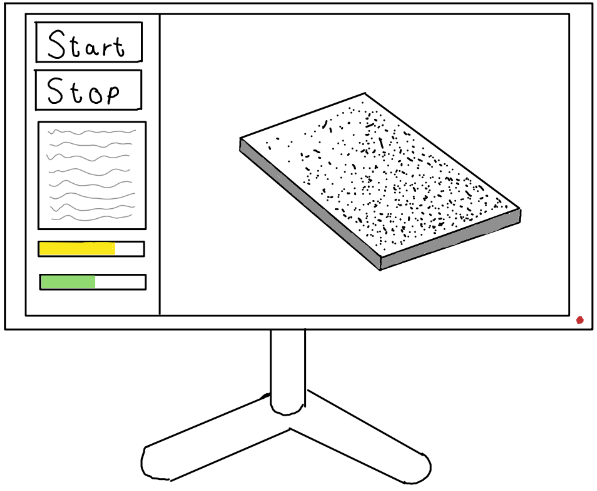
\includegraphics[width=.98\linewidth]{Sections/5 Konceptgenerering/Media/Computer.png} \\ \lillacircny \ \blueboxny \ \cyanboxny \ \blueangleny \ \greenangleny} & \makecell{Touch \\  skærm \\ \includegraphics[width=.98\linewidth]{Sections/5 Konceptgenerering/Media/Touch skærm.png} \\ \gulangleny \ \orangeangleny \ \pinkstarny \ \redkantnyy \ $ \protect\mathcolor{BrickRed}{\spadesuit}$}  &  \\ \specialrule{1pt}{0pt}{0pt}

        %Formanalyse af emne
        \rotatebox[origin=c]{90}{\cellcolor{aaublue} \textcolor{white}{\textbf{Kalibrering i forhold til  emne}}} & \makecell{Laser \\ 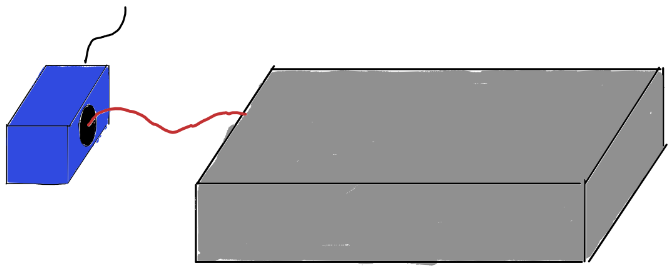
\includegraphics[width=0.98\linewidth]{Sections/5 Konceptgenerering/Media/Laser.png} \\ \lillacirc \ \gulangle \ \lillacircny \ \gulangleny} & \makecell{Kamera \\ 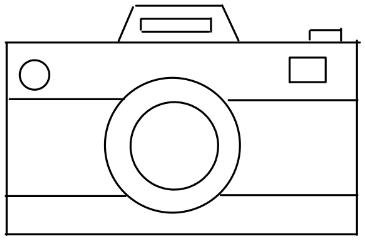
\includegraphics[width=0.8\linewidth]{Sections/5 Konceptgenerering/Media/Kamera.png} \\ \bluebox \ \orangeangle \ \blueboxny \ \orangeangleny} & \makecell{ Kontakt \\ med emnet \\ 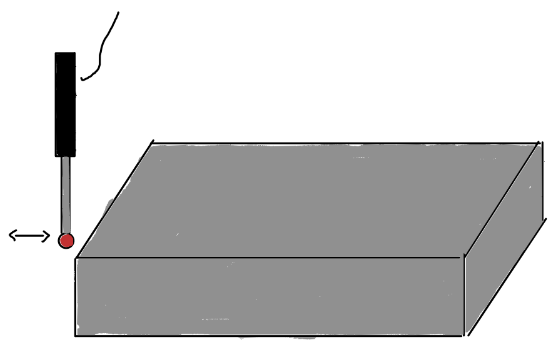
\includegraphics[width=0.98\linewidth]{Sections/5 Konceptgenerering/Media/Kontakt.png} \\ \cyanbox \ \pinkstar \ \cyanboxny \ \pinkstarny} & \makecell{Indtast på \\ computer \\ 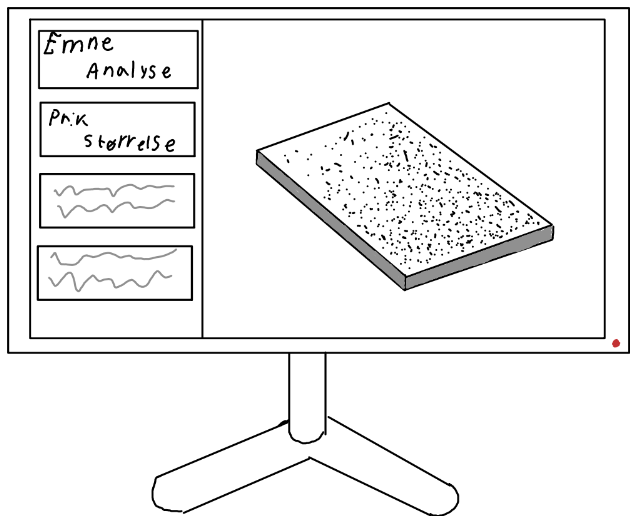
\includegraphics[width=0.98\linewidth]{Sections/5 Konceptgenerering/Media/formanalyse compu.png} \\ \blueangle \ \redkant \ \blueangleny \ \redkantnyy} & \makecell{Sensor der \\ påsættes \\ 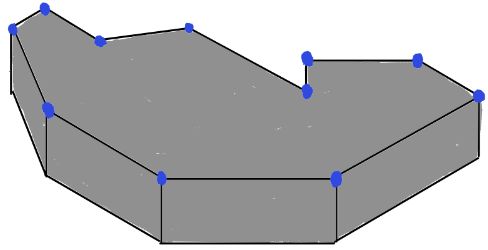
\includegraphics[width=0.98\linewidth]{Sections/5 Konceptgenerering/Media/sensor i punkt.png} \\ \greenangle \ $\protect\mathcolor{BrickRed}{\clubsuit}$ \ \greenangleny \ $\protect\mathcolor{BrickRed}{\spadesuit}$ }  \\ \specialrule{1pt}{0pt}{0pt}
 
    \end{tabular}
    \label{tab: morfologisk analyse af kontrolsystem}
\end{table}

